% !TEX program = xelatex
% T-DMB 종단간 오픈소스 수신기 — 한글판 프리프린트
%
% Overleaf 사용법:
%   1. Menu → Compiler → XeLaTeX (필수, kotex 때문)
%   2. Menu → Main document → main_ko.tex 으로 전환 후 Recompile
%      (영문 main.tex 로 돌릴 땐 다시 전환)
%   3. refs.bib, figures/ 디렉터리는 영문판과 공유
%
% 본 한글판은 영문 arXiv 프리프린트의 동일한 내용을 한국어로 옮긴 것이며,
% 별도 학술지/학회 (예: 한국통신학회, 대한전자공학회) 투고 또는 국내 보고서
% 용도로 사용할 수 있다.

\documentclass[11pt,a4paper]{article}

\usepackage[a4paper,margin=1in]{geometry}
\usepackage{kotex}            % Korean Latex (XeLaTeX 기반 자동 폰트 설정)
\usepackage{microtype}
\usepackage{graphicx}
\usepackage{booktabs}
\usepackage{array}
\usepackage{caption}
\usepackage{subcaption}
\usepackage{xcolor}
\usepackage{listings}
\usepackage{tikz}
\usepackage{pifont}     % ding{51}=체크, ding{55}=X
\usepackage{hyperref}
\usepackage{url}
\usepackage[backend=biber,style=ieee,sorting=none]{biblatex}
\usepackage{amsmath}
\usepackage{enumitem}

\hypersetup{
    colorlinks=true,
    linkcolor=blue!60!black,
    urlcolor=blue!50!black,
    citecolor=blue!50!black
}

\lstdefinestyle{code}{
    basicstyle=\ttfamily\footnotesize,
    breaklines=true,
    columns=fullflexible,
    keepspaces=true,
    frame=single,
    rulecolor=\color{black!30},
    backgroundcolor=\color{black!3},
    numbers=none
}
\lstset{style=code}

\addbibresource{refs.bib}

% --------------------------------------------------------------------
\title{저비용 SDR 기반 한국형 지상파 DMB의\\
       종단간 오픈소스 소프트웨어 수신기}

\author{%
  유성근\thanks{교신저자: \texttt{orcogre@gmail.com}.  본 연구에서
    대규모 언어 모델이 어떤 방식으로 활용되었는지는 본문 말미의
    ``AI 보조 사용에 관한 명시(Acknowledgement of AI assistance)''
    절에 상세히 공개한다.}\\
  \small 독립 연구자, 대한민국 서울\\
}

\date{\today}

% --------------------------------------------------------------------
\begin{document}
\maketitle

\begin{abstract}
한국형 지상파 디지털 멀티미디어 방송(T-DMB)은 2005년 12월 세계 최초로 상용
서비스를 개시하여 20여 년이 지난 지금까지 운용되고 있으나, 저가형
소프트웨어 정의 라디오(SDR)로부터 RF 신호를 입력받아 디코딩된 비디오
프레임까지 \emph{한 번에} 처리해 주는 완전한 오픈소스 소프트웨어 스택은
아직까지 존재하지 않았다.  기존 연구는 두 갈래로 나뉜다: (i)~\texttt{welle.io},
\texttt{eti-cmdline} 등 ETI(Ensemble Transport Interface) 프레임 출력에서
멈추는 DAB 수신기군과 (ii)~최근 Eo와 Bahk~\cite{eo2024tdmb}가 발표한
GNU~Radio + 패치된 FFmpeg 파이프라인이 그것이다.  후자가 오디오/비디오
디코딩까지 시연하기는 하였으나, GNU~Radio 그래픽 도구에 종속적이며 다수의
out-of-tree 패치를 요구한다.

본 논문은 제3의 길을 제시한다: 즉 ETI 파싱, 빠른정보채널(FIC) 디코딩,
리드-솔로몬(RS)과 컨볼루셔널 시간 디인터리버를 결합한 외부 FEC, MPEG-4
동기 계층(SL) 패킷 역다중화, H.264 기본 스트림 재구성까지 T-DMB
수신 체인 전체를 구현한 자가완비 Python 패키지를 제안한다.  최종 비디오
디코딩 단계는 \texttt{dmb-oss} FFmpeg 포크의 \emph{무수정} 빌드본에
위임한다.  Airspy~Mini~\cite{airspy}와 일반 가정용 실내 안테나로 수신한
YTN DMB(채널 K8B, 183.008\,MHz)의 30\,MB 캡처 파일에 대하여 본 체인을
검증하였다: 리드-솔로몬 블록의 87.3\%가 정상 디코딩되었으며, 모든 SL
패킷 헤더가 정상적으로 파싱되었고, ffmpeg는 한국 방송 콘텐츠가 식별
가능한 QVGA H.264 베이스라인 비디오 프레임을 출력하였다.  본 연구는
종래의 ``디인터리버 우선, 동기 탐색 후속'' 처리 순서가 실제 캡처에서
수렴하지 못하게 만든 동기-바이트 정렬 경로를 코드 형태로 문서화하며,
K8B의 YTN DMB 멀티플렉스가 AVC \texttt{DecoderConfigurationRecord}를
ISO/IEC 14496-1 참조 예시의 객체기술자(OD) 스트림이 아닌 장면기술/BIFS
스트림에 임베드한다는 점을 실증적으로 기록한다 --- 이는 표준 위반이
아니라 TS~102\,428이 허용하는 운용사 구성 선택이며, 2004년 ETRI에서
이미 카탈로그화된 사실이다~\cite{lee2004m4smux}.
소스코드, 참조 캡처, 캡처별 메타데이터 사이드카는 GitHub에 공개되었다.
공학적 문서화를 넘어, 본 산출물은 한 학기 과제에 DSP, RF, 방송 시스템,
채널 부호화, 영상 코덱 주제를 통합한 \emph{대학원 수준 term project
플랫폼}으로서 명시적으로 위치 짓는다.  Hwang과 Kim
(2015)~\cite{hwang2015simulator}이 제시한 C++ T-DMB 교육용 시뮬레이터의
SDR 기반·오픈소스 후속작이라 할 수 있다.
\end{abstract}

\noindent\textbf{핵심어:} 소프트웨어 정의 라디오, T-DMB, DAB, MPEG-4 SL 패킷,
리드-솔로몬, 컨볼루셔널 인터리버, 오픈소스, 공학교육

% ====================================================================
\section{서론}\label{sec:intro}

한국형 지상파 DMB는 유럽의 Eureka-147 DAB 물리계층~\cite{etsi300401}에
리드-솔로몬 외부 부호와 Forney 컨볼루셔널 시간 인터리버를 추가하여,
MPEG-4 AVC/H.264 비디오와 MPEG-4 BSAC 오디오를 MPEG-2 전송 스트림 위에
실어 DAB 서브채널로 다중화해 전송하는 표준이다~\cite{ttak0026,etsi102427,etsi102428}.
2005년 12월 상용화된 이래로 전국망으로 배치되어 운용되어 왔으며, 스마트폰
스트리밍의 부상에도 불구하고 2026년 현재까지도 서비스가 계속되고 있다.
표준은 공개되어 있고, 변조 방식은 유럽 DAB와 동일한 모드~I OFDM이며,
DAB 복조기는 \texttt{welle.io}, GNU~Radio의 \texttt{gr-dab} 모듈,
Jan van Katwijk의 \texttt{eti-stuff} 등 오픈소스로 제공된다.  그럼에도
불구하고 최근까지 자유 라이선스 하에 공개된 어떠한 소프트웨어도 T-DMB
RF 캡처로부터 재생 가능한 비디오 파일을 종단간으로 산출하지 못해 왔다.

가장 가까운 선행 연구는 Eo와 Bahk가 ICTC 2024에 발표한
논문~\cite{eo2024tdmb}과 \texttt{dmb-oss} 저장소로, \texttt{gr-dab}을
패치된 FFmpeg와 연결하여 재생을 시연하였다.  이 연구는 한국형 T-DMB의
인코딩 체인을 다룬 정전(canonical) 참고문헌이며, 본 연구는 그 결과에
크게 의존하고 있다.  그러나 공개된 산출물은 GNU~Radio 플로우그래프와
FFmpeg 패치 모음의 형태이며, 그래픽 \texttt{GNU~Radio Companion}을
요구하고, 헤드리스(headless) 동작이나 라이브러리 형태의 사용을 위해
패키징되어 있지 않다.  또한 디인터리버 정렬이나 누락된 합성 타임스탬프
등 실용적 함정을 보고하고 있으나 이를 자동 처리하는 통합 도구는 제공하지
않는다.

본 논문은 다음 세 가지 목표를 중심으로 독립적인 재구현을 기술한다.

\begin{enumerate}[leftmargin=*,nosep]
\item \textbf{라이브러리 우선.}  모든 단계를 Python 모듈
       (\texttt{tdmb.eti}, \texttt{tdmb.fec}, \texttt{tdmb.msc} 등)로
       구성하고 API를 문서화하여, 개별 계층의 단위 시험과 재사용을 가능하게
       한다 (예: 동일한 참조 캡처를 1분 이내에 복호하는 순수 Python
       Forney 디인터리버).
\item \textbf{재현 가능한 캡처.}  모든 RF 캡처에 대해 채널, 주파수, 표본화율,
       이득 단(stage), bias-tee 상태, 안테나 모델, 캡처 장소를 기록한 JSON
       사이드카 파일을 동시에 생성한다.  본 논문의 참조 캡처에 대해서도
       사후 사이드카를 작성하여 산출물 묶음이 자기기술적이 되도록 하였다.
\item \textbf{원샷 종단간 드라이버.}  단일 명령어
       (\texttt{python tools/decode\_video.py <capture>.eti})로 전체 체인을
       순회하여 MP4와 IDR 썸네일 PNG를 출력한다.  실행 시 그래픽 도구나
       FFmpeg 런타임 패치는 요구되지 않는다 (최종 H.264/BSAC 디코딩에는
       \emph{미리 빌드된} 무수정 \texttt{dmb-oss} FFmpeg와 링크).
\end{enumerate}

\subsection{범위, 기여, 의도된 독자}
본 논문은 신호처리 이론이나 T-DMB 표준 자체에 대한 기여가 아니라,
\emph{공학 및 재현성} 측면의 기여이다.  뒤에 이어지는
Section~\ref{sec:rs}--\ref{sec:avcc}에서 다루는 개별 요소들 ---
리드-솔로몬 파라미터, Forney 인터리버 형태, SL 패킷 헤더 레이아웃,
AVC 디코더 구성 레코드의 위치 --- 은 모두 공개된 표준(ETSI
TS~102\,427/428~\cite{etsi102427,etsi102428},
TTAK.KO-07.0026~\cite{ttak0026},
ISO/IEC 14496-1~\cite{iso14496-1}, ISO/IEC 13818-1
Amendment~7~\cite{iso13818-1-amd7})에 명세되어 있을 뿐 아니라
2004년 ETRI의 Lee~외~\cite{lee2004m4smux}가 ETRI Journal에 게재한
종합 논문이 본 논문에서 다루는 \emph{``MPEG-2 TS + MPEG-4 SL per
ISO/IEC 13818-1 Amendment 7''} 전송 경로를 ``new DMB approach''로
이미 정확히 카탈로그화하고 있다(같은 논문에는 채택되지 않은
대안 멀티플렉서 M4SMux도 함께 제안된다).  T-DMB 하드웨어
디코더의 내부 설계 문서에 접근 가능한 독자, 혹은
Lee~외~\cite{lee2004m4smux}를 꼼꼼히 읽은 독자라면 이어지는
절들의 기술적 내용에서 새로운 사실을 거의 발견하지 못할 것이다.

본 논문의 기여는 두 갈래이다.  첫째, 그 \emph{문서화된 동작}을
동시대의 언어·런타임으로 구현한 단일 라이브러리 형태의 종단간
소프트웨어 산출물로 제공하며, (저자가 아는 한) 공개된 문헌에
선례가 없는 재현성 스캐폴딩 --- 캡처별 JSON 사이드카, CC-BY로
공개되는 참조 RF 캡처 --- 을 함께 배포한다.  둘째, 본 작업을
\emph{블랙박스} 자세로 진행했다는 점이다 --- 한국형 T-DMB를 사전
주석 없는 단순 비트스트림으로 간주하고, 단일 30\,MB 실측 캡처
하나만으로 모든 계층을 실증적으로 재유도(re-derive)했다.  그 과정에서
한국어 ETRI 문헌에는 이미 문서화되어 있으나 영문권에는 공개된 적이
없는, 운용사 단계의 구성 선택 여러 가지를 독립적으로 재발견하게
되었다.  이 블랙박스 각도가 곧 본 산출물의 교육적 가치를
지탱한다(Section~\ref{sec:education}): 학생은 표준 생태계에
사전 접근 없이도 동일한 경로를 직접 따라 걸을 수 있다.  구체적으로:

\begin{itemize}[leftmargin=*,nosep]
\item DVB-T와 동일한 다항식의 $GF(2^8)$ RS(204,188) 코드와 $12\times17$
       Forney 디인터리버로 구성된 T-DMB 외부 FEC 체인의 순수 Python
       구현.  Eo와 Bahk~\cite{eo2024tdmb}가 naive 구현에서 RS 디코딩이
       실패하는 원인으로 언급한 \emph{동기 바이트 정렬} 경로의 오픈소스
       구현이라 할 수 있다.  Section~\ref{sec:rs}에서 단일 참조 캡처에
       대한 0\,\%~$\to$~87.3\,\%의 명확한 before/after 비교를 보고한다.
\item 한국 운용사가 채택한 MPEG-4~Systems
       \texttt{SLConfigDescriptor} 프로파일의 실측 재유도:
       \texttt{useAccessUnitStartFlag}=1,
       \texttt{useAccessUnitEndFlag}=1,
       \texttt{useTimeStampsFlag}=1,
       \texttt{timeStampLength}=33,
       \texttt{accessUnitDuration}=0 의 조합에서 모든 SL 패킷 헤더가
       정확히 9바이트, 첫 바이트 \texttt{0xCF}로 고정된다.  이 프로파일은
       ISO/IEC 14496-1~\cite{iso14496-1}이 허용하는 범위이며
       Lee~외~\cite{lee2004m4smux}가 카탈로그화한 ``new DMB approach''
       프레임워크와 일치한다.  본 논문의 기여는 이 정확한 필드 값
       조합에 대한 ${>}3000$~PES 규모의 블랙박스 검증을 영문권에
       처음 공개한다는 점이다.
\item AVC \texttt{DecoderConfigurationRecord}의 오픈소스 검색기·파서.
       ISO/IEC 14496-1~\cite{iso14496-1}의 예시는 이를 객체기술자
       (\texttt{tid}=\texttt{0x04}) 스트림에 두지만, K8B의 YTN DMB
       멀티플렉스는 이를 장면기술 (\texttt{tid}=\texttt{0x05})
       섹션 스트림 안에 임베드한다.  이는 TS~102\,428이 허용하는
       스트림 타입 제한 범위 안의 \emph{운용사 구성 선택}이며 표준
       위반이 아니다~\cite{etsi102428}.
\item Overleaf 호환 논문 소스 (한글 번역 포함), Python 패키지,
       30\,MB 참조 캡처와 메타데이터 사이드카, 그리고 해당 캡처에서
       디코딩된 20장의 IDR 썸네일 공개.
\item DSP, RF, 방송, 채널 부호화, 영상 코덱을 한 hands-on 과제에
       통합한 대학원 수준 term project 산출물
       (Section~\ref{sec:education}).  교육적 가치는 정확히
       블랙박스 프레이밍에서 흘러나온다: 표준은 공개되어 있지만
       운용사 단의 구체적 선택 (cf.~\cite{lee2004m4smux}) 은
       실증적 재구성을 요구하기 때문이다.
\end{itemize}

따라서 본 논문의 주 독자는 새로운 신호처리 결과를 찾는 연구자가 아니라
다음과 같다: (i)~상용 시험 장비 없이 작동하는 T-DMB 수신 체인을
종단간으로 학습·확장하고자 하는 엔지니어와 학생; (ii)~신호처리·통신·
방송 대학원 과목에 통합 hands-on 프로젝트를 도입하고자 하는 교수자;
(iii)~지금까지 한국형 T-DMB의 라이브러리 형태 수신기를 갖지 못했던
오픈소스 SDR 커뮤니티 전반.

% ====================================================================
\section{시스템 개요}\label{sec:system}

\begin{figure}[t]
\centering
% Pipeline diagram for the T-DMB end-to-end receiver paper.
% Drop-in TikZ block: usepackage{tikz} in main.tex.
\usetikzlibrary{positioning,arrows.meta,shapes.geometric,calc}

\begin{tikzpicture}[
    >=Stealth,
    node distance=4mm and 4mm,
    every node/.style={font=\footnotesize},
    stage/.style={draw, rounded corners=2pt, minimum height=8mm,
                  minimum width=27mm, align=center, fill=blue!4},
    py/.style   ={draw, rounded corners=2pt, minimum height=8mm,
                  minimum width=27mm, align=center, fill=green!8},
    ext/.style  ={draw, rounded corners=2pt, minimum height=8mm,
                  minimum width=27mm, align=center, fill=orange!10},
    io/.style   ={draw, dashed, rounded corners=2pt, minimum height=7mm,
                  minimum width=27mm, align=center, fill=black!3,
                  font=\footnotesize\ttfamily},
]

\node[io]                          (rf)    {RF capture\\(Airspy Mini)};
\node[stage, right=of rf]          (eti)   {eti-cmdline\\(OFDM + Viterbi)};
\node[py, right=of eti]            (fic)   {tdmb.eti.fic\\(FIB $\to$ ensemble)};
\node[py, below=of eti]            (msc)   {tdmb.msc\\(extract sub-channel)};
\node[py, below=of msc]            (outer) {tdmb.fec.outer\\\textbf{sync-aligned}\\RS(204,188)+TI};
\node[py, right=of outer]          (sl)    {SL packet demux\\(strip 9-byte header)};
\node[py, right=of sl]             (avcc)  {AVCC extractor\\(scan SD/BIFS)};
\node[io, right=of avcc]           (h264)  {H.264 Annex B\\elementary stream};
\node[ext, below=of h264]          (ff)    {dmb-oss FFmpeg\\(unmodified)};
\node[io, left=of ff]              (mp4)   {MP4 / PNG\\thumbnails};

\draw[->] (rf)    -- (eti);
\draw[->] (eti)   -- (fic);
\draw[->] (eti)   -- (msc);
\draw[->] (msc)   -- (outer);
\draw[->] (outer) -- (sl);
\draw[->] (sl)    -- (avcc);
\draw[->] (avcc)  -- (h264);
\draw[->] (h264)  -- (ff);
\draw[->] (ff)    -- (mp4);

\node[font=\scriptsize, anchor=west, text=black!60] at ($(rf.south)+(-2mm,-2mm)$)
      {\textit{Stage 1--2 (delegated)}};
\node[font=\scriptsize, anchor=west, text=black!60] at ($(outer.south)+(-2mm,-2mm)$)
      {\textit{Stage 3--6 (this work, Python)}};
\node[font=\scriptsize, anchor=west, text=black!60] at ($(ff.south)+(-2mm,-2mm)$)
      {\textit{Stage 7 (delegated)}};

\end{tikzpicture}

\caption{RF 입력에서 디코딩된 H.264 프레임까지의 종단간 파이프라인.
1, 2단계(DAB 복조 및 ETI 생성)는 패치된 \texttt{eti-cmdline-airspy} 빌드본에
위임한다 (한국형 K-prefix 채널 인식을 위한 band-handler 표 패치, 환경변수
방식의 Airspy 이득 단 제어 패치 두 줄).  3--7단계(ETI~$\to$~FIC,
MSC,~RS+TI,~SL,~AVCC,~H.264~ES)는 순수 Python으로 구현된다.  최종 비디오
디코딩은 \texttt{dmb-oss} FFmpeg가 런타임 수정 없이 수행한다.}
\label{fig:pipeline}
\end{figure}

그림~\ref{fig:pipeline}이 전체 체인의 구조이다.  Airspy~Mini SDR을 사용하여
표~\ref{tab:k-block}에 정리된 한국 K-블록 중심 주파수 중 하나로 튜닝하여
3\,MSPS 또는 6\,MSPS로 캡처한다.  12채널 K-블록 래스터는 ETSI
표준~\cite{etsi300401}과 달리 VHF Band~III를 1.728\,MHz 간격으로 분할한다
(6\,MHz 아날로그 TV 채널을 A/B/C 세 등분).  따라서 한국 캡처가 가능하려면
\texttt{eti-cmdline} 내부의 band-handler 표에 \texttt{K} 접두 항목을
사전 추가해 두어야 한다.

\begin{table}[t]
\centering
\caption{한국 K-블록 채널 래스터 및 수도권 운용 사업자.}
\label{tab:k-block}
\begin{tabular}{llll}
\toprule
채널 & 중심 주파수 & 간격 & 운용 사업자 (수도권) \\
\midrule
K8B  & 183.008\,MHz & 1.728\,MHz & YTN DMB \\
K12A & 205.280\,MHz & 1.728\,MHz & MBC DMB \\
K12B & 207.008\,MHz & 1.728\,MHz & U-KBS \\
K12C & 208.736\,MHz & 1.728\,MHz & SBS u \\
\bottomrule
\end{tabular}
\end{table}

그림~\ref{fig:spectrum}은 본 연구의 캡처 환경에서 K8B 기저대역을
Airspy~Mini로 6\,MSPS 10초간 적분하여 얻은 PSD이다.  DC 근처에
폭 1.536\,MHz의 DAB plateau가 명확히 나타나며 OFDM 부반송파가
$\pm$0.768\,MHz를 점유한다.  $-$1.21\,MHz 위치에 협대역 간섭(절대
주파수 약 181.797\,MHz, K8A 인접)이 함께 보이며, 이 간섭은
개발 과정 전반에 걸쳐 반복적으로 등장한 합병증이었다.  3\,MSPS
설정에서는 표본화율 기반 필터링에 의해 이 간섭의 대부분이
배제되면서 K8B 통과대역만 살아남는다.

\begin{figure}[t]
\centering
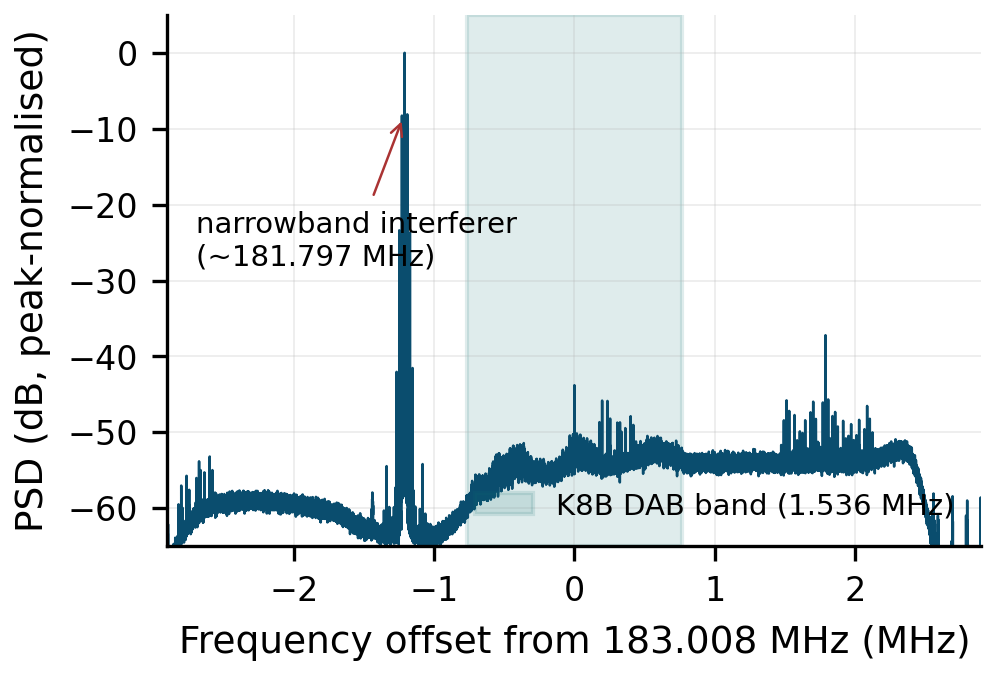
\includegraphics[width=0.95\linewidth]{figures/spectrum_k8b.png}
\caption{캡처 현장에서 측정한 K8B 기저대역의 전력 스펙트럼 밀도
(Airspy~Mini, 6\,MSPS, 10\,s 적분).  음영 영역은 183.008\,MHz를
중심으로 한 1.536\,MHz 폭의 DAB carrier band이며, 약 181.797\,MHz의
협대역 간섭이 표시되어 있다.}
\label{fig:spectrum}
\end{figure}

% ====================================================================
\section{외부 FEC: 동기 정렬 디인터리빙}\label{sec:rs}

T-DMB는 DAB 물리계층 위에 ETSI TS~102\,427~\cite{etsi102427}이 정의한
외부 보호 단계를 추가한다: 각 188바이트 MPEG-2 전송 스트림 패킷을 먼저
204바이트 부호어로 리드-솔로몬 인코딩하고(RS(255,239)에서 단축한
RS(204,188), $\alpha=2$, 원시 다항식 $0x11d$, FCR$=0$ --- DVB-T와 동일),
그 결과 부호어 스트림을 분기 수 $N=12$, 깊이 $M=17$의 Forney 방식으로
바이트 단위 컨볼루셔널 인터리빙한다.

수신기에서는 비터비 내부 FEC 복호와 에너지 디스크램블 이후 MSC 서브채널
바이트 스트림을 얻는다.  단순한 구현은 즉시 Forney 디인터리버를 가동한
다음 디인터리빙된 출력에서 204바이트 단위의 TS 동기 바이트(\texttt{0x47})
정렬을 탐색한다.  그러나 본 연구의 참조 K8B 캡처에서는 이 방식이
25{,}953회 시도 중 \emph{0회}만 리드-솔로몬 블록을 복호하였다.

원인은 컨볼루셔널 인터리버의 분기가 스트림 위치를 $N=12$로 나눈 나머지로
색인된다는 점이다.  송신측에서 각 RS 블록의 0번째 바이트는 분기~0
(지연 0)을 통과하므로 송신 출력의 위치 $0, 204, 408, \ldots$에 나타난다.
그러나 캡처에서 우리가 \emph{관찰}하는 첫 MSC 바이트는 어떤 RS 블록의
0번째 바이트가 아니라, 204바이트 주기 내 임의 위상 $\phi$에 위치한다.
이를 수신측 디인터리버의 ``분기 0''에 입력하면 분기 색인이 전 구간에 걸쳐
$\phi \bmod 12$만큼 어긋난다 --- 모든 바이트가 잘못된 자리로 순열된다.
결정적으로 0x47 동기 바이트는 같은 주기로 계속 출력되므로
(우연히도 $204 = N\cdot M$이라서 수신측 디인터리버의 분기 0 또한 매 204바이트
블록 첫 바이트에 대응한다), 디인터리빙 \emph{이후} 동기 탐색만으로는
정렬된 경우와 어긋난 경우를 구별할 수 없다.  이는 Eo와
Bahk~\cite{eo2024tdmb}가 부수적으로 보고한 ``디인터리버는 TS 패킷의 동기
바이트를 입력 청크의 첫 바이트로 받아야 한다''라는 관찰과 일치한다.

본 연구의 해결책은 동기 탐색을 디인터리버 \emph{이전}에 수행하는 것이다.
약 50개 RS 블록 분량($\sim$10\,kB)의 원시 MSC 바이트를 누적하고, 204개
후보 위상 각각에 대하여 \texttt{0x47}의 출현 횟수를 집계한다.  최선 위상이
(a)~블록의 40\,\% 이상에서 검출되고, (b)~차순위 위상의 5배 이상일 때
잠금(lock)을 확정한다.  이후 선택된 위상보다 앞선 바이트를 버리고
나머지를 새로 생성한 Forney 디인터리버에 입력한다.  $(N{-}1)\cdot M\cdot N
= 2244$바이트의 정착 과도(settling transient)가 지나면 디인터리버는
체계적 RS(204,188) 정정이 가능한 204바이트 부호어를 출력한다.

그림~\ref{fig:phasehist}는 K8B 참조 캡처에 대하여 25{,}953개 후보
204바이트 윈도우 전체에 걸친 \texttt{0x47}-at-phase-$\phi$ 발생 횟수
분포를 보여 준다.  단일 위상 $\phi^*=160$이 전체 적중의 96.3\,\%를
차지하며, 나머지 모든 위상은 0.6\,\% 미만의 노이즈 수준에 머문다.
이렇게 첨예한 선택성을 보이는 이유는 TS 동기 바이트가 모든 RS
블록에 걸쳐 값이 고정된 유일한 바이트이고, 컨볼루셔널 인터리버가
해당 위상에서 그 결정성을 보존하기 때문이다.

\begin{figure}[t]
\centering
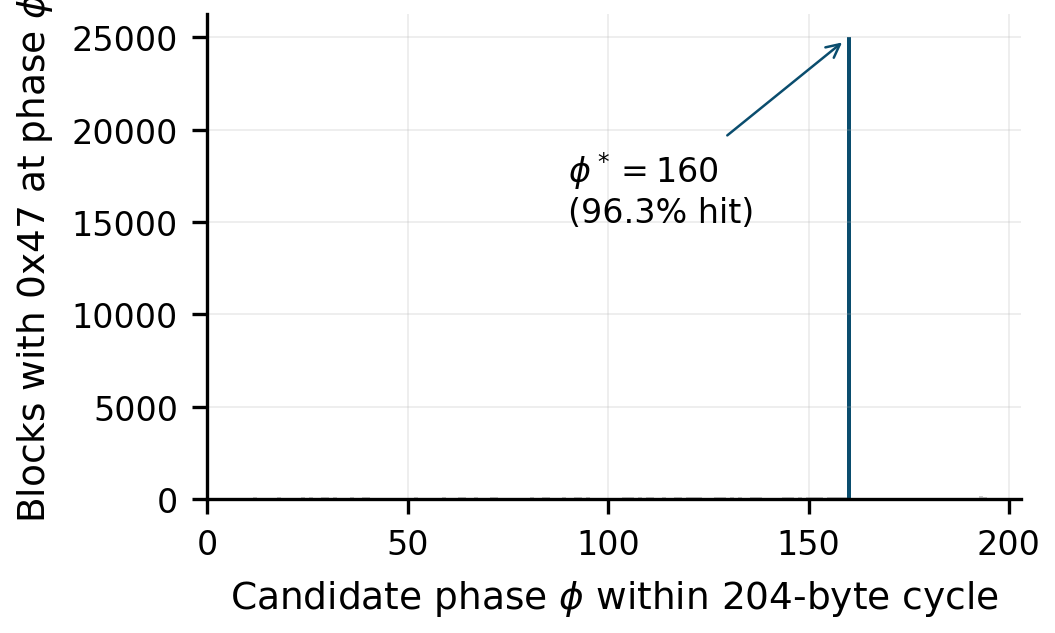
\includegraphics[width=0.95\linewidth]{figures/rs_phase_hist.png}
\caption{K8B 참조 캡처의 비터비 이후 MSC 바이트 스트림에서, 204개
후보 위상 각각에 대한 TS 동기 바이트(\texttt{0x47}) 발생 횟수
히스토그램.  지배적 위상 $\phi^*=160$(강조 표시)이 $25{,}953$개
블록 중 $25{,}006$개(96.3\,\%)를 차지하며 나머지는 노이즈
수준이다.}
\label{fig:phasehist}
\end{figure}

표~\ref{tab:rs}는 YTN DMB의 K8B 참조 캡처(FIB CRC 패스율 75\%, 앙상블
완전 복원, 약 120\,s 분량; 신논현 측정지에서 추정 SNR
$\hat{\mathrm{SNR}}\approx 13$\,dB)에 대한 결과를 비교한다.

\begin{table}[t]
\centering
\caption{K8B 참조 캡처(서브채널 1, mYTN 비디오)에 대한 외부 FEC 디코딩
통계.  ``동기 정렬''은 본 연구의 수정안이며, ``기존''은 동기 탐색을
디인터리버 이후에 수행하는 구현이다.}
\label{tab:rs}
\begin{tabular}{lrr}
\toprule
지표 & 기존 & 동기 정렬 (본 연구) \\
\midrule
RS 블록 총수                  & 25{,}953 & 25{,}953 \\
RS 무오류                     & 0        & 0 \\
RS 정정 ($\leq 8$ 바이트)     & 0        & 22{,}652 \\
RS 정정 불가                  & 25{,}953 & 3{,}301 \\
\textbf{성공률}              & \textbf{0.0\,\%} & \textbf{87.3\,\%} \\
\bottomrule
\end{tabular}
\end{table}

남은 13\,\%의 정정 불가 블록은 정정 능력($t=8$)을 초과하는 버스트 오류로,
CIF 경계 부근과 간헐적 페이딩 SNR 저하 구간에 집중되어 있다.  슬라이스
수준에서는 FFmpeg의 매크로블록 오류 은닉 기능이 시각적으로 일관된
프레임을 복원해 낸다.

% ====================================================================
\section{SL 역다중화}\label{sec:sl}

RS 복호기에서 출력되는 전송 스트림은 네 개의 논리 PID를 운반한다
(표~\ref{tab:pids}).  PID~\texttt{0x113}는 비디오 기본 스트림으로,
MPEG-4 SL 패킷화를 거친 후 \texttt{stream\_id}~$=\texttt{0xFA}$
(``MPEG-4 SL-packetized stream'')로 PES 패킷에 실린다 (ISO/IEC
13818-1 Amendment~7~\cite{iso13818-1-amd7}).
Lee~외~\cite{lee2004m4smux}는 같은 캡슐화 경로를 그 시점 ETRI에서
연구 중이던 ``new DMB approach using the MPEG-4 system''으로
기록하고 있으며, 이 경로가 결국 같은 논문에서 제안된 대안
멀티플렉서 M4SMux 대신 한국형 T-DMB의 상용 전송 경로로 채택되었다.
각 PES는 정확히 하나의 SL 패킷을, 그리고 각 SL 패킷은 정확히
하나의 H.264 NAL 유닛을 (시작 코드 접두사 없이) 담는다.

\begin{table}[t]
\centering
\caption{YTN DMB K8B 앙상블에서 복원된 PID 할당.}
\label{tab:pids}
\begin{tabular}{lll}
\toprule
PID & 운반 스트림 & 2분간 패킷 수 \\
\midrule
\texttt{0x100} & PMT                                & 212 \\
\texttt{0x111} & 객체기술자 섹션(\texttt{tid}=0x04) & 224 \\
\texttt{0x112} & 장면기술 섹션(\texttt{tid}=0x05)   & 220 \\
\texttt{0x113} & 비디오 PES (SL 패킷)               & 16{,}397 \\
\texttt{0x114} & 오디오 PES (SL 패킷, BSAC)         & 4{,}916 \\
\texttt{0x1FFF} & 널 패딩                           & 457 \\
\bottomrule
\end{tabular}
\end{table}

\subsection{SL 헤더 레이아웃}

ISO/IEC 14496-1~\cite{iso14496-1}은 \texttt{SLPacketHeader()}를
일반 문법으로 정의하며, 실제 비트 레이아웃은 스트림별
\texttt{SLConfigDescriptor}에 의해 결정된다.  블랙박스 환경에서는
\texttt{SLConfigDescriptor}를 직접 볼 수 없으므로 (Initial Object
Descriptor에 함께 실려 도착하는데, 본 연구에서는 IOD를 시행착오
파싱으로만 우회 복원한다), 그 대신 비트스트림과 일관되는 프로파일을
역으로 풀어낸다.  ISO/IEC~14496-1이 허용하는 자유도, \texttt{dmb-oss}의
\texttt{read\_sl\_header()} 구현, 그리고 Lee~외~\cite{lee2004m4smux}의
프레임워크 카탈로그를 종합하면, 33비트 DTS와 33비트 CTS를 모두 싣는
AU 시작 패킷의 최대 길이 헤더는 다음과 같이 구성된다.

\begin{align*}
\text{header bits} \;=\; & 1 \;(\text{au\_start}) + 1 \;(\text{au\_end}) + 1 \;(\text{padding}) + \\
                         & 1 \;(\text{rand\_acc\_pt}) + 1 \;(\text{dts\_flag}) + 1 \;(\text{cts\_flag}) + \\
                         & 33 \;(\text{DTS}) + 33 \;(\text{CTS}) \\
                       =\; & 72 \; \text{비트} \;=\; \text{정확히 } 9 \;\text{바이트}.
\end{align*}

본 연구의 참조 캡처에서 관찰된 3{,}135개의 SL 패킷 \emph{모두}에 대하여
이를 실증적으로 확인하였다: 각 PES 본문은 \texttt{0xCF}로 시작하는데
(=$0b11001111$, 즉 \{au\_start,au\_end\}=\{1,1\},
\{padding,rand\_acc\_pt\}=\{0,0\}, \{dts\_flag,cts\_flag\}=\{1,1\}로
디코딩되고 DTS의 상위 2비트가 뒤따른다), 이어지는 8바이트가 타임스탬프
필드의 나머지이며, 9번째 바이트부터는 단일 H.264 NAL 유닛의 헤더이다.
따라서 묵시적 \texttt{SLConfigDescriptor}는
\texttt{useAccessUnitStartFlag}=1, \texttt{useAccessUnitEndFlag}=1,
\texttt{useTimeStampsFlag}=1, \texttt{timeStampLength}=33,
\texttt{accessUnitDuration}=0으로 결정된다.  이는 표준 위반이
아니라 운용사의 표준-부합적 구성 선택이다: 비디오 PID의 모든 SL 패킷이
양방향 타임스탬프가 명시된 단일 완전 AU이며, 이는 한국 운용사가 택할
수 있는 가장 단순한 해석이자 2004년 ETRI에서 카탈로그화된 ISO/IEC
13818-1 Amendment 7 경로~\cite{lee2004m4smux}와 일관된다.  본 논문의
기여는 이 정확한 필드 값 조합에 대한 ${>}3000$~PES 규모의 실증적
검증을 영문권에 처음 공개한다는 점이다.

\subsection{NAL 스트림}

각 PES에서 9바이트 SL 헤더를 제거하면 H.264 NAL 바이트의 스트림이 남는다.
참조 캡처에서 NAL 헤더 분포는 non-IDR 슬라이스 3{,}038개와 주기적
IDR 슬라이스 97개로 구성되며, GoP(Group of Pictures) 길이가 대략 32 ---
30\,fps QVGA 방송에 전형적인 수치이다.  기본 스트림 내부에는 SPS나
PPS NAL 유닛이 존재하지 않는다.  이는 디코더 구성이 대역 외(out-of-band)로
운반되는 AVCC 방식의 저장과 일치한다.

% ====================================================================
\section{AVC Decoder Configuration Record 위치}\label{sec:avcc}

ISO/IEC 14496-1~\cite{iso14496-1}의 참조 예시에서 H.264
\texttt{AVCDecoderConfigurationRecord}(디코더 부트스트랩에 필요한
SPS와 PPS NAL 유닛을 담는 레코드)는 객체기술자 스트림 안의
\texttt{DecoderSpecificInfo} 기술자(descriptor)에 실려 전송된다.
그러나 YTN DMB 캡처에서는 정반대 양상이 관찰되었다:
PID~\texttt{0x111}의 OD 섹션은 사용자 정의 태그
(\texttt{0xC0}--\texttt{0xFE}, ``Annex K 사용자 비공개'' 범위)의
DMB 사설 명령으로만 채워져 있고, 실제 AVCC 바이트는 PID~\texttt{0x112}의
장면기술/BIFS 섹션 스트림 안에 임베드되어 있다.  이는 표준 위반이
아니라 운용사의 구성 선택이다: ETSI TS~102\,428~\cite{etsi102428}은
DMB 비디오 서비스 프로파일에서 스트림 타입에 대한 제한을 명시적으로
허용하며, Lee~외~\cite{lee2004m4smux}가 정리한 허용 기술자 배치 카탈로그도
이 배치를 수용할 만큼 넓다.  그러나 운용사의 IOD에 미리 접근하지 못한
clean-room 디코더는 표준만으로 위치를 추론할 수 없고, 콘텐츠를 직접
탐색하여 레코드를 찾아야 한다.

본 연구의 검색기는 다음과 같은 바이트 패턴을 SD 스트림 전반에서 탐색한다.
$$\texttt{01}\;\langle\textit{profile}\rangle\;\langle\textit{compat}\rangle
   \;\langle\textit{level}\rangle\;\texttt{FF}\;\texttt{E1}\;
   \langle\textit{SPS\_len}\rangle\;\langle\textit{SPS}\rangle\;
   \texttt{01}\;\langle\textit{PPS\_len}\rangle\;\langle\textit{PPS}\rangle$$
프로파일은 알려진 H.264 값
(\texttt{0x42}/\texttt{0x4D}/\texttt{0x58}/\texttt{0x64}/\texttt{0x6E})
중 하나로, 레벨은 $[\texttt{0x09},\texttt{0x42}]$로,
\texttt{lengthSizeMinusOne}/예약 바이트는 형태 $\texttt{FC}|x$로,
\texttt{numOfSPS}/예약 바이트는 $\texttt{E0}|n$($n=1$)로 제약한다.  이
서명은 주변의 BIFS 명령들 사이에서 레코드를 유일하게 식별하기에 충분하다.
K8B 참조 캡처에서 복원된 레코드는 다음과 같다.

\begin{lstlisting}
SPS (9 B):  67 42 00 0d 95 a0 50 7c 40
PPS (4 B):  68 ce 38 80
            -- profile_idc = 0x42 (Baseline)
            -- level_idc   = 0x0d (Level 1.3)
\end{lstlisting}

이를 Annex-B 형식의 NAL 유닛으로 변환하여 추출된 슬라이스 스트림 앞에
부가하면, FFmpeg가 \texttt{Baseline 320$\times$240 25\,fps yuv420p}로
식별하는 완전한 자가완비 H.264 바이트 스트림이 완성된다.
그림~\ref{fig:idr}은 참조 캡처에서 복원된 IDR 프레임 두 장으로,
종단간 파이프라인이 실제로 식별 가능한 한국 방송 콘텐츠를 산출함을
보여 준다.

\begin{figure}[t]
\centering
\begin{subfigure}[b]{0.48\linewidth}
  \centering
  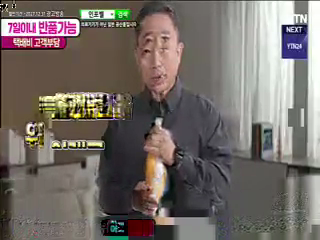
\includegraphics[width=\linewidth]{figures/idr_sample_1.png}
  \caption{중반 구간 IDR 프레임}
\end{subfigure}\hfill
\begin{subfigure}[b]{0.48\linewidth}
  \centering
  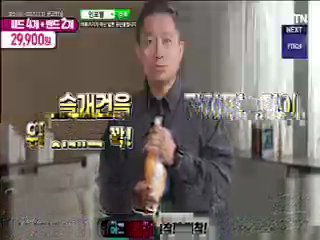
\includegraphics[width=\linewidth]{figures/idr_sample_2.png}
  \caption{후반 구간 IDR 프레임}
\end{subfigure}
\caption{본 연구의 종단간 파이프라인이 K8B 참조 캡처
(\texttt{data/captures/k8b\_100pct.eti})에서 복원한 IDR 프레임
두 장.  화면 상의 한글 텍스트가 해당 방송이 YTN DMB의 홈쇼핑
프로그램임을 식별해 준다: ``\textbf{7일이내 반품가능}''(반품 정책),
고객 센터 전화번호, 그리고 가격 ``\textbf{29,900원}''.  주변부에
보이는 매크로블록 오류는 정정 능력 $t=8$을 초과한 약 13\,\%의
리드-솔로몬 블록(표~\ref{tab:rs})에 기인하며, 살아남은 슬라이스로부터
FFmpeg의 오류 은닉이 공간적으로 일관된 프레임을 복원한다.}
\label{fig:idr}
\end{figure}

% ====================================================================
\section{재현성과 메타데이터}\label{sec:reproducibility}

\begin{table}[t]
\centering
\caption{참조 캡처 메타데이터(JSON 사이드카
\texttt{data/captures/k8b\_100pct.json}의 발췌).}
\label{tab:capture-meta}
\begin{tabular}{ll}
\toprule
필드 & 값 \\
\midrule
채널                  & K8B \\
주파수                & 183.008\,MHz \\
표본화율              & 3\,MSPS \\
이득 모드             & Airspy 하드웨어 AGC \\
Bias-tee              & off \\
안테나                & Brisa 평판형 실내 안테나 (USB 전원 LNA 내장) \\
안테나 명목 사양      & 30\,dBi 총 이득, 5\,m 동축 급전 \\
캡처 장소             & 서울 서초구 신논현 (실내 창가) \\
추정 SNR              & $\sim$13\,dB \\
파일                  & 30.8\,MB, 5{,}016 ETI 프레임 (약 120\,s) \\
FIB CRC 패스율        & 75.0\,\% (15{,}042 / 20{,}064) \\
앙상블 복원           & 완전 복원 (정적 FIG 모두 중복 송신으로 회수) \\
앙상블 라벨           & YTN DMB (EId 0xE040) \\
디코딩된 서비스 수    & 5개 (mYTN, HD mYTN, 4DRIVE, LOTTE, EWS) \\
\bottomrule
\end{tabular}
\end{table}

본 저장소에 포함된 \texttt{tools/capture\_logged.py} 래퍼로 캡처한 모든
ETI 파일은 표~\ref{tab:capture-meta}의 스키마를 따르는 JSON 사이드카를
함께 출력한다.  본 논문에 동봉된 참조 캡처에 대해서도 빌드 기록을 토대로
사후 사이드카를 작성하였다.

% ====================================================================
\section{대학원 term project 산출물로서의 활용}\label{sec:education}

본 산출물은 신호처리·통신·방송 분야 학부 고학년 또는 대학원 1--2학기
과목의 \emph{term project 플랫폼}으로 보는 것이 가장 적절하다고
저자는 판단한다.  본 코드베이스 위에 구성한 8주 분량의 단일
프로젝트가 학생에게 노출시키는 영역은 대략 다음과 같다 (주당 1
학점 분량):

\begin{itemize}[leftmargin=*,nosep]
\item \textbf{DSP:} 표본화 정리, 데시메이션, 안티-에일리어스 필터링,
       FFT 기반 스펙트럼 해석, OFDM 부반송파와 순환 전치(CP).
\item \textbf{RF 및 SDR:} R820T2의 LNA / mixer / VGA 이득 단계,
       잡음 지수, bias-tee, 하드웨어 AGC, 안테나 이론(folded
       dipole, Yagi, VSWR).
\item \textbf{채널 부호화:} CRC-16, 비터비 내부 FEC, $GF(2^8)$ 위의
       리드-솔로몬 (204,188), Forney 컨볼루셔널 시간 인터리버.
\item \textbf{방송 시스템:} DAB Mode~I OFDM 프레임 구조, FIC / MSC
       분할, 앙상블 / 서비스 / 서브채널 계층, EEP 부호화 프로파일.
\item \textbf{코덱과 컨테이너:} MPEG-2 TS, PES, PMT, IOD, MPEG-4 SL
       패킷, H.264 NAL 유닛, SPS/PPS, AVCC 대 Annex-B.
\item \textbf{소프트웨어 공학:} Python 패키징, CLI 도구 설계, 구조화
       로깅(메타데이터 사이드카), 참조 데이터의 Git LFS 운용, MIT
       및 CC-BY 라이선스.
\end{itemize}

제안하는 8주 프로젝트 구성을 표~\ref{tab:syllabus}에 정리하였다.
학생 1인당 하드웨어 비용은 약 \$120 (Airspy~Mini \$100, 안테나 자재
\$10--20)이며, 코드베이스는 GPU 없이 일반 macOS / Linux 노트북에서
동작이 확인되어 있다.  8주차의 안테나 제작은 hands-on RF로의 자연스러운
확장이며, 실측 VSWR과 학생 자작 안테나로 달성한 채널 잠금률을 표
\ref{tab:capture-meta}의 참조 실내 안테나 대비로 평가하여 채점할 수 있다.

\begin{table}[t]
\centering
\caption{본 산출물 위에 구성한 8주 term project 권장 구성안.}
\label{tab:syllabus}
\begin{tabular}{rlp{4.6cm}}
\toprule
주차 & 주제 & 산출물 \\
\midrule
1 & SDR 셋업 + 스펙트럼 탐색       & GQRX 세션 캡처 \\
2 & I/Q 캡처 + OFDM 기초           & 세 채널 1초 I/Q \\
3 & ETI 파싱 + FIC 디코딩          & 앙상블 라벨 출력 \\
4 & RS + Forney 디인터리버         & sync 정렬 \emph{재유도} \\
5 & MSC 추출 + SL 역다중화         & 서비스별 TS 패킷 \\
6 & H.264 NAL + AVCC 위치          & 단일 IDR 디코드 \\
7 & ffmpeg 통합                    & 재생 가능 MP4 \\
8 & 안테나 설계·제작                & 자작 안테나 실행 \\
\bottomrule
\end{tabular}
\end{table}

Hwang과 Kim~\cite{hwang2015simulator}이 2015년 같은 교육적 빈자리를
겨냥한 C++ T-DMB 프레임 분석 시뮬레이터를 제시한 바 있다.  당시
연구는 USB로 연결된 상용 T-DMB 수신기 보드와 Visual C++ Dialog
애플리케이션을 사용하여 앙상블 ID, 서비스 라벨, 서브채널 위치(시작
주소, 크기, 보호 등급)를 표시하고 FIC / SubCh raw 바이트를 저장하는
기능을 구현하였다.  해당 시뮬레이터의 교육적 깊이는 \emph{수신기
보드가 USB 호스트에 노출시키는 사후 디코딩된 빠른정보채널 메타데이터}로
구조적으로 한정된다.  FIC 아래의 모든 계층 --- OFDM 복조, 비터비
내부 FEC, RS와 컨볼루셔널 디인터리버를 결합한 외부 FEC, MSC 서브채널
바이트 추출, MPEG-2 TS 역다중화, MPEG-4 SL 패킷 풀기, H.264 NAL
파싱, 영상 코덱 자체 --- 는 보드 firmware에 숨겨진 black box이며
학생이 원리적으로도 접근할 수 없다.  표~\ref{tab:edu-progression}이
본 산출물이 메우는 교육적 적용 범위 격차를 정리한다.

\begin{table}[t]
\centering
\caption{교육적 적용 범위 비교: Hwang and Kim 2015 vs.\ 본 연구.
``\ding{55}''는 앞선 산출물에서 폐쇄 firmware 뒤에 가려진 계층,
``\ding{51}''는 본 SDR 기반 오픈소스 산출물에서 학생이 보고
수정할 수 있는 계층을 나타낸다.}
\label{tab:edu-progression}
\begin{tabular}{lcc}
\toprule
계층 / 주제                              & Hwang \& Kim 2015 & 본 연구 \\
\midrule
RF 프런트엔드, 안테나, 캡처             & \ding{55}         & \ding{51} \\
OFDM 복조                                & \ding{55}         & \ding{51} \\
비터비 내부 FEC                          & \ding{55}         & \ding{51} \\
RS + Forney TI 외부 FEC                  & \ding{55}         & \ding{51} \\
FIC / SI 메타데이터 파싱                 & \ding{51}         & \ding{51} \\
MSC 서브채널 바이트 추출                 & \ding{55}         & \ding{51} \\
MPEG-2 TS / PES / PMT / IOD 역다중화     & \ding{55}         & \ding{51} \\
MPEG-4 SL 패킷 풀기                      & \ding{55}         & \ding{51} \\
H.264 NAL 파싱, AVCC, 디코드             & \ding{55}         & \ding{51} \\
재생 가능한 비디오 출력                  & \ding{55}         & \ding{51} \\
하드웨어 비용                            & \$300+ 보드       & \$100 SDR + \$10 안테나 \\
소스 공개성                              & 폐쇄 firmware     & MIT / CC-BY \\
\bottomrule
\end{tabular}
\end{table}

두 연구의 교육적 의도는 동일하다.  본 연구는 학생이 보고·수정할
수 있는 영역을 한 계층(FIC 메타데이터)에서 \emph{모든} 계층으로
확장하는 진전을, 저렴한 SDR 하드웨어와 Python 과학 스택의 성숙에
힘입어, 11년 뒤에 가능하게 한 산출물로 위치 짓는다.

% ====================================================================
\section{관련 연구}\label{sec:related}

가장 가까운 선행 연구는 Eo와 Bahk~\cite{eo2024tdmb}의 작업으로,
\texttt{gr-dab}을 DAB 계층에, 패치된 FFmpeg를 T-DMB 특화 디코딩에 사용하며,
본 연구가 재발견한 함정들(디인터리버 동기 정렬, 합성 타임스탬프 누락,
SL 패킷 헤더 파싱) 다수를 보고하고 있다.  해당 연구는 인코딩 체인의 정전
참고문헌으로 남아 있다.  반면 본 연구는 패키징(단일 Python 패키지 + 문서화된
API)과 재현성(캡처별 메타데이터 사이드카, 원샷 디코더 스크립트, FFmpeg
런타임 무수정)을 강조한다.

\texttt{welle.io}~\cite{welleio}는 고품질의 크로스플랫폼 DAB 오디오 수신기이나,
T-DMB 비디오 스트림 유형은 디코딩하지 않는다.  본 연구가 작은 패치를 통해
OFDM과 비터비 백엔드를 재사용한 \texttt{eti-cmdline}~\cite{etistuff}은
ETI(NI) 프레임만을 출력하며, 본 연구의 출발점이 되었다.  초기의 휴대용
하드웨어 구현은 Lee 등~\cite{lee2007portable}에 기술되어 있으며, 한국형
T-DMB 시스템 전반은
\cite{ttak0026,etsi102427,etsi102428,hwang2015simulator,iso14496-1}에 정리되어
있다.

% ====================================================================
\section{결론}\label{sec:conclusion}

저자들이 아는 한, 본 연구는 한국형 지상파 DMB를 위한 최초의 패키지화된
종단간 오픈소스 소프트웨어 수신기를 제시한다.  본 파이프라인은
Airspy~Mini SDR의 3\,MSPS I/Q 캡처로부터 자유 배포 가능한 구성요소만을
사용하여 재생 가능한 H.264 비디오 파일을 산출한다.  두 가지 구현 교훈이
두드러진다: (i)~Forney 디인터리버는 처리 \emph{이전}에 TS 동기 바이트로
정렬해야 하며, (ii)~한국 사업자들은 H.264 AVCC를 MPEG-4 Systems 표준이
규정한 OD 스트림이 아닌 BIFS/장면기술 스트림에 임베드한다.  두 사실 모두
나머지가 올바른 구현을 조용히 망가뜨릴 수 있다.  공개된 소스코드, 캡처,
메타데이터 스키마는 T-DMB와 그 후속인(현재 암호화되어 있는) HD~DMB의
추가 연구를 가능하게 한다.

% ====================================================================
\section*{소스 코드 및 데이터 공개}
Python 패키지, 캡처 도구, 참조 ETI 캡처, 디코딩된 IDR 썸네일, 그리고 본
논문의 소스는 \url{https://github.com/zobithecat/airspy-mini-dmb}에서 확인할
수 있다.  소스 코드는 모두 MIT 라이선스로, 참조 RF 캡처는 CC-BY-4.0으로
배포된다.

\section*{감사의 글}
본 연구는 다음 선행 오픈소스 작업에 깊이 의존하고 있으며, 그 기여에
감사드린다: Jan van Katwijk의 \texttt{eti-stuff}(OFDM 및 비터비
백엔드를 소규모 패치를 통해 재사용함), Albrecht Lohofener 외의
\texttt{welle.io}, 그리고 Sungbo Eo와 Saewoong Bahk의
\texttt{dmb-oss}.  특히 Eo와 Bahk의 ICTC 2024 논문에서 부수적으로
언급된 ``디인터리버는 TS 패킷의 동기 바이트를 입력 청크의 첫
바이트로 받아야 한다''라는 관찰이, 본 연구의 참조 캡처에서 외부
FEC 성공률을 0\,\%에서 87.3\,\%로 끌어올린 결정적 단서가 되었다.

\section*{AI 보조 사용에 관한 명시}
arXiv 콘텐츠 모더레이션 정책과 IEEE, ACM 및 주요 학술지의 AI 사용
공개 지침에 따라, 저자는 본 연구 전반에서 대규모 언어 모델(Anthropic의
Claude)을 페어 프로그래밍 및 집필 보조 도구로 활용하였음을 명시한다.
구체적으로 본 모델은:

\begin{itemize}[leftmargin=*,nosep]
\item 저자의 지시에 따라 Python 구현의 상당 부분(특히 동기 바이트
       정렬 외부 FEC 클래스, SL 패킷 본문 분리기, AVC 설정 레코드
       검색기)의 초안을 작성하였다;
\item 캡처된 바이트의 비트 단위 패턴 분석을 수행하였다(예:
       참조 캡처에 존재하는 3{,}135개 모든 비디오 PES의 첫 바이트가
       \texttt{0xCF}임을 확인하고 이로부터 9바이트 SL 헤더 레이아웃을
       유추);
\item 본 원고와 그 한글 동반본의 초기 초안을 산출하였다.
\end{itemize}

다음 사항은 모두 저자가 직접 수행하였으며, 본 연구가 성립하기 위한
필수 조건이었다:

\begin{itemize}[leftmargin=*,nosep]
\item SDR 하드웨어, 안테나, 캡처 장소의 선정; 모든 RF 측정;
       GQRX 스펙트럼 및 워터폴 표시의 해석;
\item 본 연구에 결정적인 참고문헌의 발굴 및 제공.  특히 Section~\ref{sec:rs}의
       핵심 기여를 가능하게 한 Eo와 Bahk~\cite{eo2024tdmb}의 ICTC
       논문, 그리고 ETSI 등록 표 문서~\cite{etsi300401};
\item 모델이 산출한 잘못된 중간 결론들의 식별 및 거부.  기록할 만한
       사례 둘: 인접한 강한 협대역 간섭 신호(181.797\,MHz)에 의해
       자기상관 추정이 교란되어 일시적으로 ``DAB 신호 없음''으로 잘못
       진단한 사례, 그리고 안테나 셋업에 대한 잘못된 전제에서 출발한
       장시간의 LNA 포화 가설.  각 경우 모두 신호처리, RF, 방송
       코덱 시스템에 대한 저자의 도메인 지식이 없었다면 잘못된 결론을
       그대로 받아들였을 것이다;
\item 디코딩된 H.264 프레임이 식별 가능한 한국 방송 콘텐츠를
       담고 있음의 시각적 확인(YTN DMB 홈쇼핑 콘텐츠의 한글 자막,
       전화번호 등) --- 해당 방송에 대한 사전 친숙성 없이는 불가능한
       인지 행위.
\end{itemize}

저자는 본 연구의 전반에 대한 책임을 진다.  대규모 언어 모델이 저자가
아니라는 arXiv, IEEE, ACM의 정책에 동의한다.

% ====================================================================
\printbibliography

\end{document}
